\documentclass[paper]{IEEEtran}
\IEEEoverridecommandlockouts
% The preceding line is only needed to identify funding in the first footnote. If that is unneeded, please comment it out.
\usepackage[english]{babel}
\usepackage[utf8x]{inputenc}
\usepackage{amsmath}
\usepackage{graphicx}
\usepackage[colorinlistoftodos]{todonotes}
\usepackage{gensymb} % this could be problem
\usepackage{float}
\usepackage{fancyref}
\usepackage{subcaption}
\usepackage{amssymb}

\usepackage{pythonhighlight}

\usepackage{xspace}

\newcommand\nd{\textsuperscript{nd}\xspace}
\newcommand\rd{\textsuperscript{rd}\xspace}
\newcommand\nth{\textsuperscript{th}\xspace} %\th is taken already


\usepackage{xcolor}
\usepackage{listings}

\usepackage{fancyhdr}

\usepackage{karnaugh-map}

\definecolor{mGreen}{rgb}{0,0.6,0} % for python
\definecolor{mGray}{rgb}{0.5,0.5,0.5}
\definecolor{mPurple}{rgb}{0.58,0,0.82}


\definecolor{mygreen}{RGB}{28,172,0} % color values Red, Green, Blue for matlab
\definecolor{mylilas}{RGB}{170,55,241}

\lstdefinestyle{CStyle}{
    commentstyle=\color{mGreen},
    keywordstyle=\color{magenta},
    numberstyle=\tiny\color{mGray},
    stringstyle=\color{mPurple},
    basicstyle=\footnotesize,
    breakatwhitespace=false,         
    breaklines=true,                 
    captionpos=b,                    
    keepspaces=true,                 
    numbers=left,                    
    numbersep=5pt,                  
    showspaces=false,                
    showstringspaces=false,
    showtabs=false,                  
    tabsize=2,
    language=C
}


\lstset{language=Matlab,%
    %basicstyle=\color{red},
    breaklines=true,%
    morekeywords={matlab2tikz},
    keywordstyle=\color{blue},%
    morekeywords=[2]{1}, keywordstyle=[2]{\color{black}},
    identifierstyle=\color{black},%
    stringstyle=\color{mylilas},
    commentstyle=\color{mygreen},%
    showstringspaces=false,%without this there will be a symbol in the places where there is a space
    numbers=left,%
    numberstyle={\tiny \color{black}},% size of the numbers
    numbersep=9pt, % this defines how far the numbers are from the text
    emph=[1]{for,end,break},emphstyle=[1]\color{red}, %some words to emphasise
    %emph=[2]{word1,word2}, emphstyle=[2]{style},    
}



\makeatletter
\renewcommand\paragraph{\@startsection{paragraph}{4}{\z@}%
            {-2.5ex\@plus -1ex \@minus -.25ex}%
            {1.25ex \@plus .25ex}%
            {\normalfont\normalsize\bfseries}}
\makeatother
\setcounter{secnumdepth}{4} % how many sectioning levels to assign numbers to
\setcounter{tocdepth}{4}    % how many sectioning levels to show in ToC



\begin{document}

\title{EE314 Digital Electronics Laboratory\\
2017-2018 Spring Term Project Proposal Report
}


\author{

\IEEEauthorblockN{1\textsuperscript{st} Halil TEMURTAS}
\IEEEauthorblockA{\textit{2094522} }
\textit{halil.temurtas@metu.edu.tr}

\and

\IEEEauthorblockN{2\textsuperscript{nd} Erdem TUNA}
\IEEEauthorblockA{\textit{2167419} }
\textit{erdem.tuna@metu.edu.tr}


}

\maketitle

\begin{abstract}

The project 

\end{abstract}

\begin{IEEEkeywords}
The, laboratory , project
\end{IEEEkeywords}

\section{Introduction}
\- \indent
	In this project, our aim is to design a oscilloscope.


\section{Project}
\- \indent


\begin{figure}[h!]
	\setlength{\unitlength}{\textwidth}
	\center 
	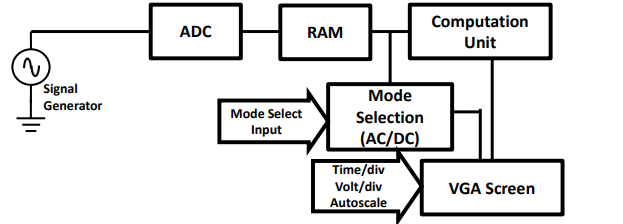
\includegraphics[width=0.47\textwidth]{block_diagram}
	\caption{\label{fig:block_diagram}The Block Diagram of the project}
\end{figure}

	 \textit{Figure~\ref{fig:block_diagram}}    

	
%\begin{figure}[h!]
%	\centering
%	\begin{subfigure}{.48\textwidth}
%		\centering
%		\includegraphics[width=1\linewidth]{scope_28_SimResult}
		%\caption{Theoretical Output of VCO.}
		%\label{fig:VCOFor1kHzTheoretical}
%	\end{subfigure}%
%	\newline
%	\begin{subfigure}{.48\textwidth}
%		\centering
%		\includegraphics[width=1\linewidth]{scope_28}
		%\caption{Practical Output of VCO.}
		%\label{fig:VCOFor1kHzPractical}
%	\end{subfigure}
	%\caption{VCO Outputs for 1kHz.}
%	\label{fig:VCOFor1kHz}
%\end{figure}

\subsection{ADC} \- \indent
	

\subsection{RAM} \- \indent

\subsection{Computation Unit} \- \indent


\subsection{Mode Selection (AC/DC)} \- \indent
	Two slide switches will be assigned to retrieve the desired mode information from the user. According to the information the screen will display according to the desired mode.

\paragraph{AC Mode} \- \indent
	In AC Mode operation of the oscilloscope, the DC offset voltage is removed from the input voltage before it is reflected to the VGA monitor. For that Computation Unit will be used to extract offset information from stored data.

\paragraph{DC Mode} \- \indent
	In DC Mode operation of the oscilloscope, the DC offset voltage is untouched from the stored data of the input voltage. The stored data is reflected directly to the VGA monitor. 
	

\subsection{VGA Screen} \- \indent

\paragraph*{Time/div Input} \- \indent

\paragraph*{Voltage/div Input} \- \indent

\paragraph*{Autoscale Input} \- \indent



\paragraph*{VGA Controller} \- \indent
	The VGA controller combines the numbers BRAM, the delta-t BRAM and the waveform to
create a signal that is displayed on the computer monitor. Each of the BRAMs contains an image
that is ready for display on the screen, but they must be positioned relative to each other and
combined. The VGA controller also provides read/write timing for other modules. Since the
BRAMs must be read 60 times per second, the VGA controller needs to send out a signal (write
warning) to warn the decimal module and the menu FSM not to write when it is reading. The
VGA controller also produces a select signal that controls which waveform BRAM is being
written to/read from.

	
	
\section{Conclusion}
\- \indent
	Conclusion
	
	

\begin{thebibliography}{00}
\bibitem{b1} J.-J. Lin, Y.-P. Li, W.-C. Hsu, and T.-S. Lee, “Design of an FMCW radar baseband signal processing system for automotive application,” SpringerPlus, vol. 5, no. 1, 2016.	
%\bibitem{b2} “LF353 Datasheet.” [Online]. Available: http://www.ti.com/lit/ds/symlink/lf353-n.pdf. [Accessed: 20-Jan-2018].
%\bibitem{b3} “2N7000 Datasheet.” [Online]. Available: https://www.onsemi.com/pub/Collateral/2N7000-D.PDF. [Accessed: 20-Jan-2018].
%\bibitem{b4} “LF353 Datasheet.” [Online]. Available: http://www.falstad.com/circuit/e-vco.html.

%\bibitem{b6} Y. Yorozu, M. Hirano, K. Oka, and Y. Tagawa, ``Electron spectroscopy studies on magneto-optical media and plastic substrate interface,'' IEEE Transl. J. Magn. Japan, vol. 2, pp. 740--741, August 1987 [Digests 9th Annual Conf. Magnetics Japan, p. 301, 1982].
%\bibitem{b7} M. Young, The Technical Writer's Handbook. Mill Valley, CA: University Science, 1989.
\end{thebibliography}




\end{document}